\documentclass{beamer}
\usepackage{listings,bm}
\usepackage{hyperref}
\usepackage{tikz}
\usetikzlibrary{positioning,shadows,arrows,shapes,calc}
\usepackage{tipa}
\newcommand{\ipa}[1]{\fontfamily{cmr}\selectfont\textipa{#1}}
\def\labelenumi\theenumi
\usepackage{graphicx}
\usepackage{amsmath}
\mode<presentation>{\usetheme{Frankfurt}}
\AtBeginSection
{
  \begin{frame}<beamer>
    \frametitle{Outline}
    \tableofcontents[currentsection,currentsubsection]
  \end{frame}
}
\title{Lecture 20: AutoVC: Zero-Shot Voice Conversion using Autoencoder Loss}
\author{Mark Hasegawa-Johnson\\These slides are in the public domain}
\date{ECE 417: Multimedia Signal Processing}
\institute{University of Illinois}
\titlegraphic{\includegraphics[width=0.3in]{exp/block-I-primary.png}}
\begin{document}

% Title
\begin{frame}
  \maketitle
\end{frame}

% Title
\begin{frame}
  \tableofcontents
\end{frame}


%%%%%%%%%%%%%%%%%%%%%%%%%%%%%%%%%%%%%%%%%%%%%%%%%%%%%%%%%
\section{Autoencoders}
\setcounter{subsection}{1}

\begin{frame}
  \frametitle{Autoencoder}
  \begin{columns}
    \begin{column}{0.5\textwidth}
      A two-layer network is a network with two matrix
      multiplications, e.g.,
      \begin{align*}
        \bm{h}&=g\left(\bm{W}_1\bm{x}\right)\\
        \bm{x'}&=\bm{W}_2\bm{h}
      \end{align*}
      An \textbf{autoencoder} is a neural net trained to minimize the
      difference between its output and its input:
      \begin{align*}
        \mathcal{L}=\Vert\bm{x'}-\bm{x}\Vert^2
      \end{align*}
    \end{column}
    \begin{column}{0.5\textwidth}
      \includegraphics[width=\textwidth]{exp/autoencoder2.png}

      \url{https://commons.wikimedia.org/wiki/File:Autoencoder_schema.png}
    \end{column}
  \end{columns}
\end{frame}

\begin{frame}
  \frametitle{Dimensionality Reduction}
  \begin{columns}
    \begin{column}{0.5\textwidth}
      Notice that if $\text{len}(\bm{h})=\text{len}(\bm{x})$, then
      there is a trivial solution:
      \begin{align*}
        \bm{h}&=\bm{I}\bm{x}=\bm{x}\\
        \bm{x'}&=\bm{I}\bm{h}=\bm{x}\\
        \mathcal{L}&=\Vert\bm{x'}-\bm{x}\Vert^2=0
      \end{align*}
      For this reason, an autoencoder is only interesting if $\bm{h}$
      is limited in some way.  Most often, it is because
      $\text{len}(\bm{h})<\text{len}(\bm{x})$.
    \end{column}
    \begin{column}{0.5\textwidth}
      \includegraphics[width=\textwidth]{exp/autoencoder2.png}

      \url{https://commons.wikimedia.org/wiki/File:Autoencoder_schema.png}
    \end{column}
  \end{columns}
\end{frame}

\begin{frame}
  \frametitle{Dimensionality reduction}
  \begin{columns}
    \begin{column}{0.5\textwidth}
      The goal of the autoencoder is to learn a vector $\bm{h}$ that
      is shorter than $\bm{x}$, but contains most of the same
      information.
    \end{column}
    \begin{column}{0.5\textwidth}
      \includegraphics[width=\textwidth]{exp/autoencoder2.png}

      \url{https://commons.wikimedia.org/wiki/File:Autoencoder_schema.png}
    \end{column}
  \end{columns}
\end{frame}


\begin{frame}
  \frametitle{Linear Autoencoder = Smart PCA}
  \begin{columns}
    \begin{column}{0.5\textwidth}
      Suppose that the hidden layer is linear, $\text{len}(\bm{h})=K$,
      $\text{len}(\bm{x})=D$, and suppose that
      $\bm{W}_1=\bm{W}_2^T=\bm{W}^T$, i.e.,
      \begin{align*}
        \bm{h}&=g\left(\bm{W}^T\bm{x}\right)\\
        \bm{x'}&=\bm{W}\bm{h}\\
        \mathcal{L}&=\Vert\bm{x'}-\bm{x}\Vert^2
      \end{align*}
      In order to minimize $\mathcal{L}$, the columns of $\bm{W}$ must
      span the same space as the first $K$ principal components.  They
      don't need to be orthogonal, but they must span the space.
    \end{column}
    \begin{column}{0.5\textwidth}
      \includegraphics[width=\textwidth]{exp/changeofbasis.png}

      \url{https://commons.wikimedia.org/wiki/File:Change_of_basis_22.svg}
    \end{column}
  \end{columns}
\end{frame}

\begin{frame}
  \frametitle{Linear Autoencoder = Smart PCA}
  \begin{columns}
    \begin{column}{0.7\textwidth}
      \begin{itemize}
      \item If $\bm{x}\in\Re^D$, then regular PCA finds the
        eigenvectors of the covariance matrix: an $\mathcal{O}\{D^3\}$
        operation.
      \item Smart PCA is $\mathcal{O}\{TNKD\}$, where $K$ is the
        number of principal components you want to find, $T$ is the
        number of training epochs, and $N$ is the number of training
        tokens.
      \item If $K\ll D$ (e.g., you have 100,000 dimensions but you
        only want 100 principal components), smart PCA can be faster
        than regular PCA.
      \end{itemize}
    \end{column}
    \begin{column}{0.3\textwidth}
      \includegraphics[width=\textwidth]{exp/autoencoder2.png}

      \url{https://commons.wikimedia.org/wiki/File:Autoencoder_schema.png}
    \end{column}
  \end{columns}
\end{frame}


\begin{frame}
  \frametitle{Types of autoencoders}

  \begin{itemize}
  \item A \textbf{linear autoencoder} finds the first $K$ principal
    components.  This architecture is sometimes called smart PCA,
    because it is faster than PCA if $K\ll D$.
  \item A \textbf{sparse autoencoder} can represent data that are
    drawn from a \textbf{sparse manifold}, which is the union of two
    or more hyperplanes.
  \item A \textbf{deep autoencoder} can represent data that are drawn
    from a \textbf{nonlinear manifold}, which is a curved
    lower-dimensional space embedded in a higher dimensional space.
  \item An \textbf{LSTM autoencoder} represents a sequence
    $[\bm{x}_1,\ldots,\bm{x}_T]$ using a shorter sequence
    $[\bm{h}_1,\ldots,\bm{h}_U]$ ($U<T$).
  \end{itemize}
\end{frame}

\begin{frame}
  \frametitle{Sparse Manifold}
  \begin{columns}
    \begin{column}{0.5\textwidth}
      A sparse manifold is the union of two or more hyperplanes.

      For example, suppose that we have a set of 3d vectors, all of
      which are drawn from one of the two planes shown at right.  How
      can we represent that?
    \end{column}
    \begin{column}{0.5\textwidth}
      \includegraphics[width=\textwidth]{exp/intersectingplanes.png}

      \url{https://commons.wikimedia.org/wiki/File:PlaneIntersection.png}
    \end{column}
  \end{columns}
\end{frame}

\begin{frame}
  \frametitle{Sparse Autoencoder/Sparse PCA}
  \begin{columns}
    \begin{column}{0.7\textwidth}
      \begin{itemize}
        \item A \textbf{sparse autoencoder} is an autoencoder in
        which $\text{len}(\bm{h})\ge\text{len}(\bm{x})$, but only the
        $K<\text{len}(\bm{x})$ largest elements of $\bm{h}$ are
        allowed to be nonzero.
      \item 
        For example, in the image at right, only the two largest
        elements of $\bm{h}$ are nonzero; the others are zeroed out.
      \item 
        The result is that $\bm{x'}=\bm{x}$ if $\bm{x}$ is on a
        plane spanned by any two of the columns of $\bm{W}$.
      \end{itemize}
    \end{column}
    \begin{column}{0.3\textwidth}
      \includegraphics[width=\textwidth]{exp/sparseautoencoder.png}

      \url{https://commons.wikimedia.org/wiki/File:Autoencoder_sparso.png}
    \end{column}
  \end{columns}
\end{frame}

\begin{frame}
  \frametitle{Nonlinear Manifold}
  \begin{columns}
    \begin{column}{0.5\textwidth}
      A nonlinear manifold is a curved lower-dimensional surface
      embedded in a higher-dimensional vector space.

      For example, the figure at right shows a 2d manifold embedded in
      a 3d vector space.
    \end{column}
    \begin{column}{0.5\textwidth}
      \includegraphics[height=0.8\textheight]{exp/kleinbottle.png}

      \url{https://commons.wikimedia.org/wiki/File:Klein_bottle.svg}
    \end{column}
  \end{columns}
\end{frame}

\begin{frame}
  \frametitle{Deep Autoencoder}
  \begin{columns}
    \begin{column}{0.5\textwidth}
      In a deep autoencoder, $\bm{z}=f(\bm{x})$ is computed by a
      network with at least two layers.  Since a two-layer network can
      compute any function, therefore $f(\bm{x})$ can be any function.

      The autoencoder loss can be zero ($\bm{x'}=\bm{x}$) whenever
      $\bm{x}$ is on a nonlinear manifold whose dimension is less than or equal
      to $\text{len}(\bm{z})$.
    \end{column}
    \begin{column}{0.5\textwidth}
      \includegraphics[width=\textwidth]{exp/deepautoencoder.png}

      \url{https://commons.wikimedia.org/wiki/File:Autoencoder_structure.png}
    \end{column}
  \end{columns}
\end{frame}

\begin{frame}
  \frametitle{LSTM Autoencoder}

  An LSTM autoencoder downsamples $[\bm{x}_1,\ldots,\bm{x}_T]$ to
  $[\bm{h}_1,\ldots,\bm{h}_U]$, then upsamples again to reconstruct $\bm{x'}$.
  
  \centerline{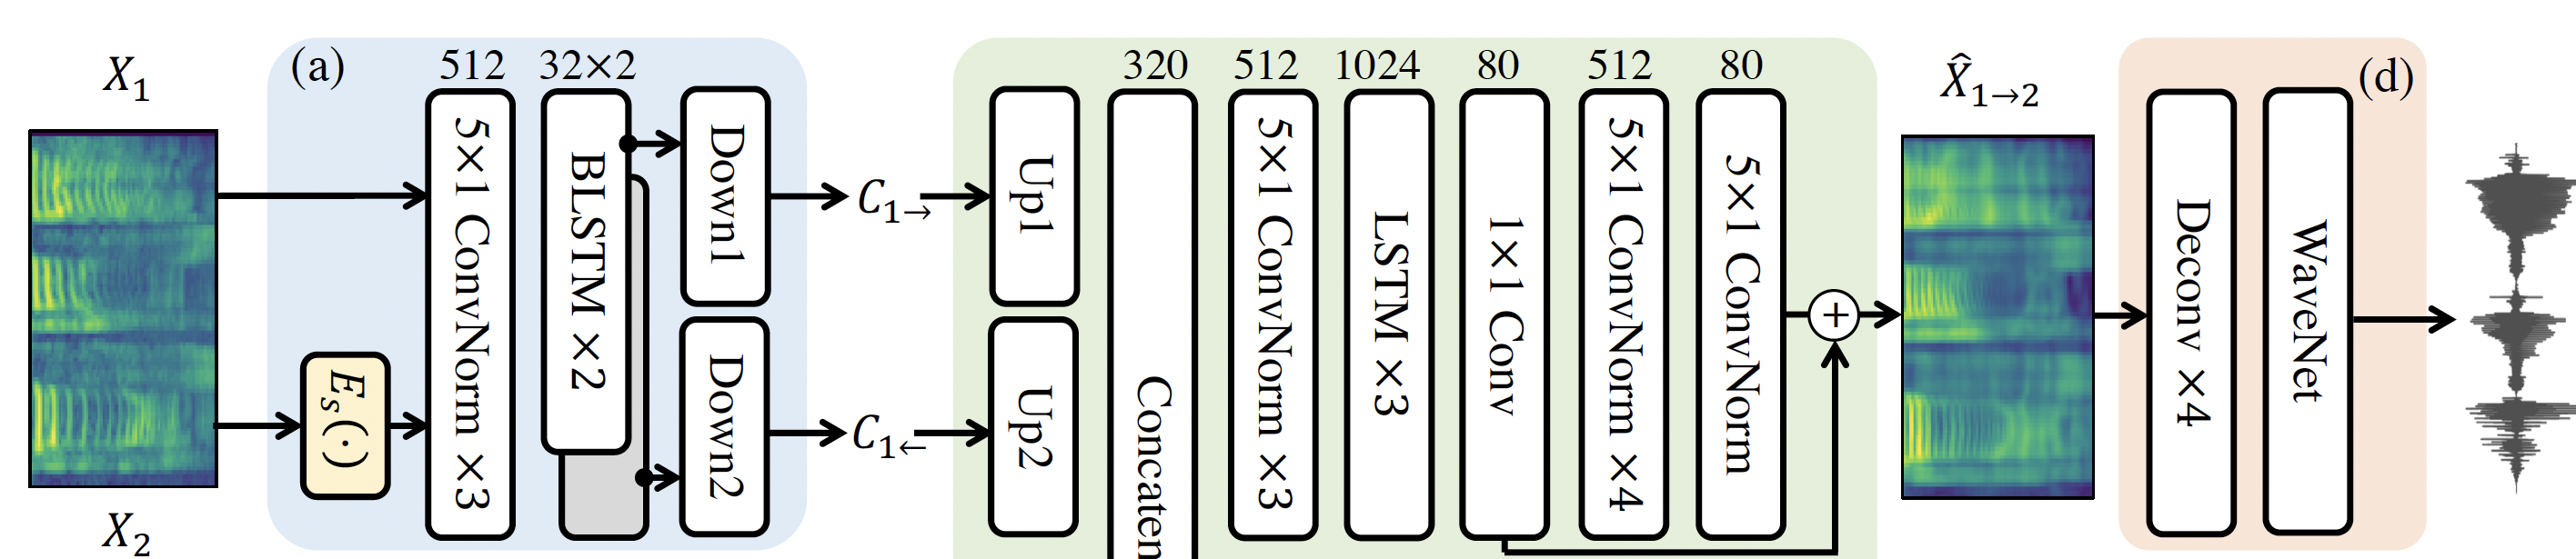
\includegraphics[width=\textwidth]{figs/lstmautoencoder.png}}

  \centerline{\url{http://proceedings.mlr.press/v97/qian19c/qian19c.pdf}}
\end{frame}

    
%%%%%%%%%%%%%%%%%%%%%%%%%%%%%%%%%%%%%%%%%%%%%%%%%%%%%%%%%
\section{Voice Conversion}
\setcounter{subsection}{1}

\begin{frame}
  \frametitle{Voice Conversion}

  \begin{itemize}
  \item Voice conversion transforms one person's speech so that it sounds like another person.
  \item Usually we transform one spectrogram to another, then use
    Griffin-Lim to reconstruct the waveform.
  \end{itemize}
\end{frame}

\begin{frame}
  \frametitle{Fully Supervised Voice Conversion}

  \begin{itemize}
    \item In fully-supervised voice conversion, we have examples of
      the source speaker and the target speaker saying the same sentences.
    \item A training example is $(\bm{X}_1,\bm{X}_2)$ where
      $\bm{X}_1=[\bm{x}_{1,1},\ldots,\bm{x}_{1,T}]$ is a source
      spectrogram and $\bm{X}_2=[\bm{x}_{2,1},\ldots,\bm{x}_{2,T}]$ is
      a target spectrogram (of another speaker saying the same thing).
      The first step is to approximately time-align them, e.g., by
      zero-padding the shorter one.
    \item Then we train a FCN, CNN, LSTM or other neural network that
      computes $\hat{\bm{x}}_{2,t}=f_t(\bm{X}_1)$, and train it to minimize
      \begin{displaymath}
        \mathcal{L}=\frac{1}{2}\Vert\bm{X}_2-\bm{X}_{1\rightarrow{2}}\Vert_F^2=
        \frac{1}{2}\sum_{t=1}^T\Vert\bm{x}_{2,t}-f_t(\bm{X}_1)\Vert^2
      \end{displaymath}
  \end{itemize}
\end{frame}

\begin{frame}
  \frametitle{Many-to-Many Voice Conversion}

  \begin{itemize}
  \item A many-to-many voice converter is trained using a database
    with many speakers.
  \item The ``content code'' $\bm{C}_1=E_C(\bm{X}_1)$ is a sequence of
    vectors specifying what the generated utterance should say.
  \item The ``speaker code'' $\bm{S}_2=E_S(\bm{X}_2)$ specifies what
    the target speakers sounds like, e.g., it might be an x-vector or
    d-vector.
  \item The generated utterance $\hat{\bm{X}}_{1\rightarrow
    2}=D(\bm{C}_1,\bm{S}_2)$ is a spectrogram with the same text
    content as $\bm{X}_1$, but sounds like the person who said $\bm{X}_2$.
  \end{itemize}
\end{frame}

\begin{frame}
  \frametitle{Many-to-Many VC Examples}

  \centerline{\url{https://auspicious3000.github.io/autovc-demo/}}
\end{frame}

\begin{frame}
  \frametitle{How to train many-to-many voice conversion}

  \begin{itemize}
  \item Fully supervised: We have a database (like
    \href{https://datashare.ed.ac.uk/handle/10283/2651}{VCTK}) in
    which each speaker says the same things, so we can train using
    \begin{displaymath}
      \mathcal{L}=\frac{1}{2}\Vert\bm{X}_2-\bm{X}_{1\rightarrow 2}\Vert_F^2
    \end{displaymath}
  \item StarGAN, AutoVC: We have a database of many speakers, but they
    are not all saying the same things, so we need to use some more
    clever training method.
  \end{itemize}
\end{frame}
    

%%%%%%%%%%%%%%%%%%%%%%%%%%%%%%%%%%%%%%%%%%%%%%%%%%%%%%%%%
\section{AutoVC}
\setcounter{subsection}{1}

\begin{frame}
  \frametitle{AutoVC: Zero-Shot Voice Conversion Using Autoencoder Loss}

  The key idea of AutoVC is that we train the network using
  self-reconstructions, $\bm{X}_{1\rightarrow
    1}=D(\bm{C}_1,\bm{S}_1)$:
  \begin{displaymath}
    \mathcal{L}=\frac{1}{2}\Vert\bm{X}_1-\bm{X}_{1\rightarrow 1}\Vert_F^2
  \end{displaymath}
  Then, during test time, we substitute in the speaker code for a
  different speaker.
  \centerline{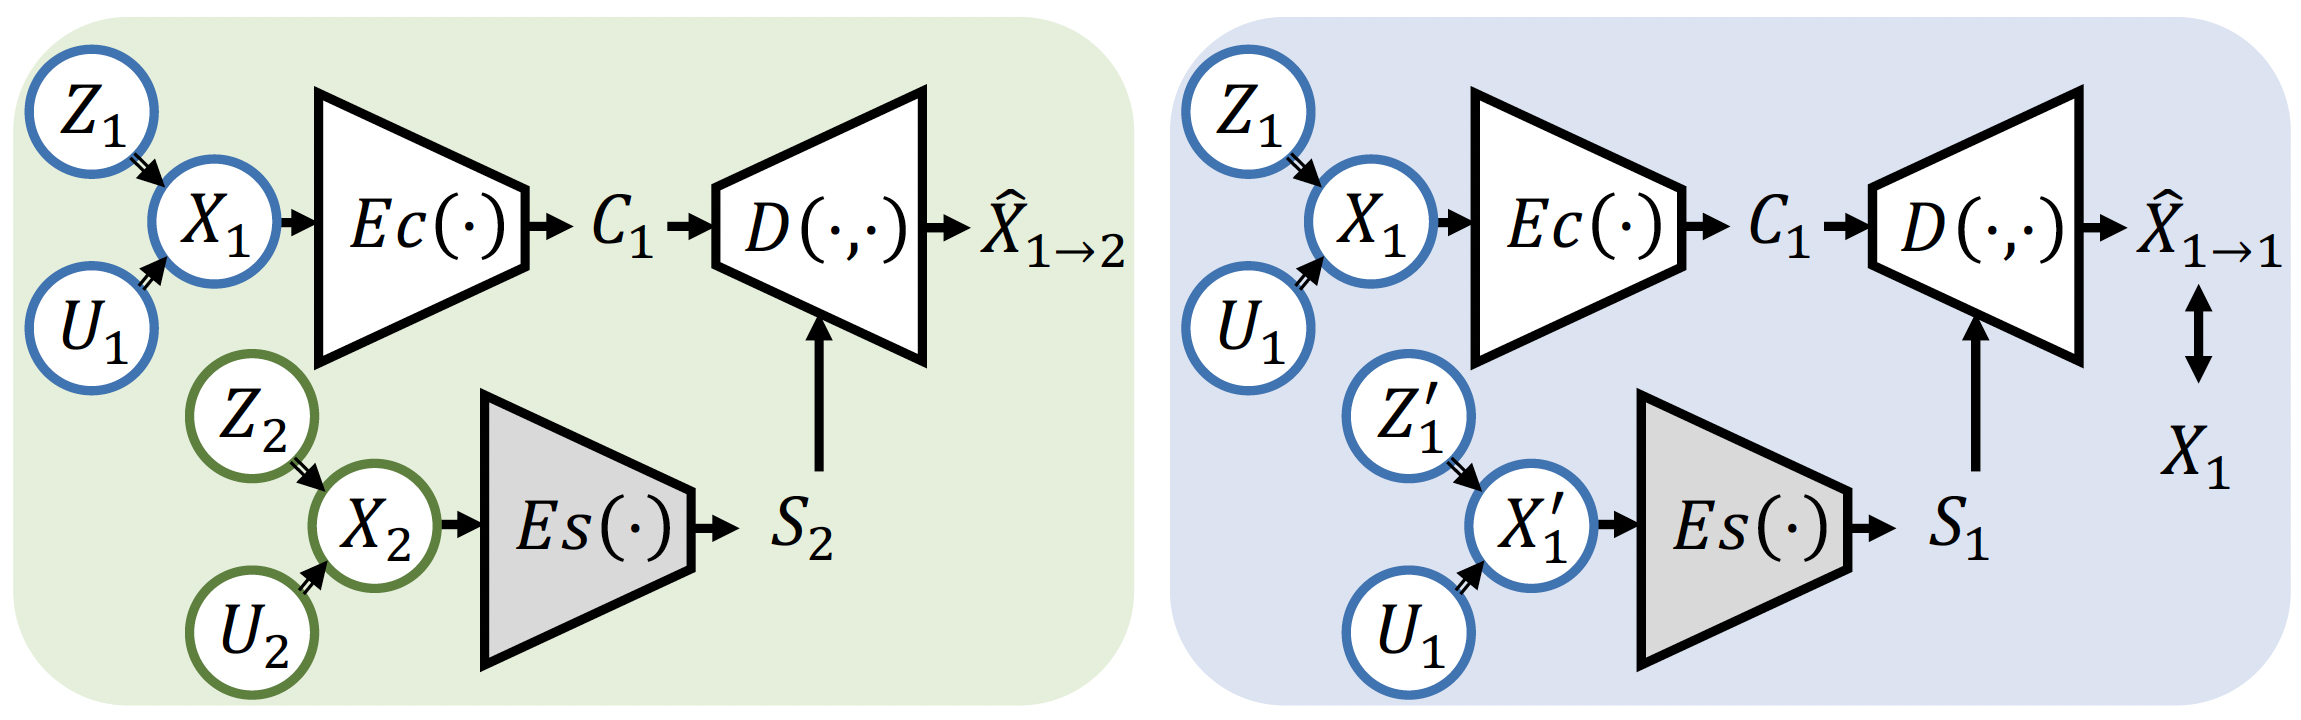
\includegraphics[width=\textwidth]{figs/qianfig1.png}}
    
\end{frame}

\begin{frame}
  \frametitle{AutoVC: How to avoid $C_1$ and $S_1$ swapping information?}

  \begin{itemize}
  \item The problem that needs to be solved is: how do we make sure
    that $\bm{S}_1$ encodes \textbf{only} information about the
    speaker, and $\bm{C}_1$ encodes \textbf{only} information about
    the content?
  \item Suppose we pre-train the speaker encoder, $\bm{S}_1$, as a
    speaker verification system.  The task of speaker verification
    works best if the utterance content has been normalized away, so
    training in this way will ensure that $\bm{S}_1$ contains no
    content information.
  \item Now we just need to remove any speaker information from the
    content code.
  \end{itemize}
\end{frame}

\begin{frame}
  \frametitle{The ``information bottleneck'' idea}

  \centerline{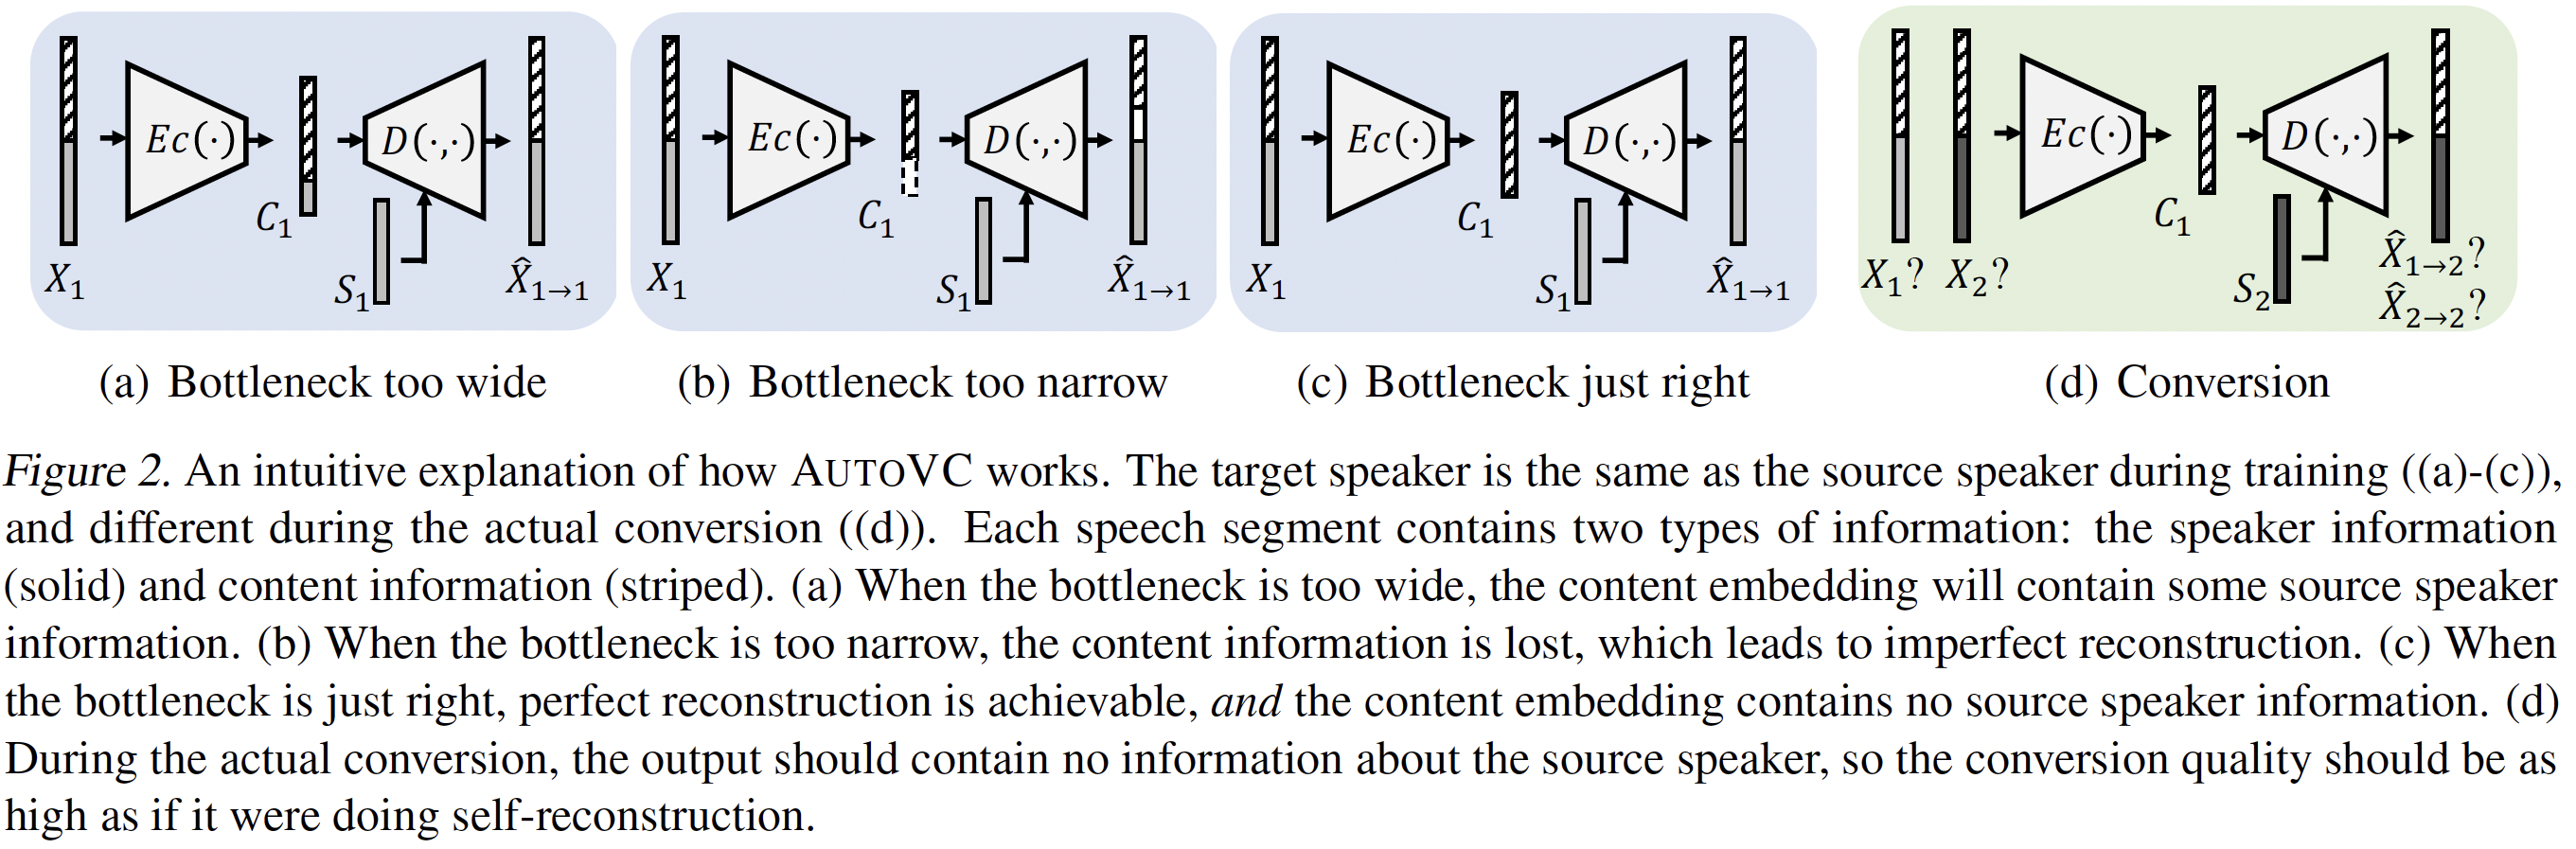
\includegraphics[width=1.1\textwidth]{figs/qianfig2.png}}
\end{frame}


\begin{frame}
  \frametitle{The ``information bottleneck'' idea}

  \begin{itemize}
  \item The input spectrogram is $\bm{X}=[\bm{x}_1,\ldots,\bm{x}_T]$,
    where each spectral vector has a dimension of $D$.
  \item The content code is $\bm{C}=[\bm{c}_1,\ldots,\bm{c}_U]$, where each
    content codevector has a dimension of $K$.
  \item The bottleneck factor, $B$, is the ratio of
    $\text{size}(\bm{C})/\text{size}(\bm{X})$, i.e.,
    \begin{displaymath}
      B = \left(\frac{K}{D}\right)\times\left(\frac{U}{T}\right)
    \end{displaymath}
  \end{itemize}
\end{frame}

\begin{frame}
  \frametitle{The ``information bottleneck'' idea}

  \begin{displaymath}
    B = \left(\frac{K}{D}\right)\times\left(\frac{U}{T}\right)
  \end{displaymath}
  \begin{itemize}
  \item When $B$ is too large, speaker information leaks into the
    content code, so a converted speech file sounds like the source
    speaker.  We can measure this using a speaker verification system:
    ask it, is this converted file the same as the source speaker?  If
    so, reduce $B$, and train again.
  \item When $B$ is too small, converted speech is unintelligible.  We
    can test this by measuring
    $\mathcal{L}=\frac{1}{2}\Vert\bm{X}_1-\bm{X}_{1\rightarrow{1}}\Vert^2$.
    If $\mathcal{L}$ is too large, increase $B$, and train again.
  \item When $B$ is just right, converted speech is intelligible, but
    sounds nothing like the source speaker.
  \end{itemize}
\end{frame}

\begin{frame}
  \frametitle{The AutoVC Architecture}

  \centerline{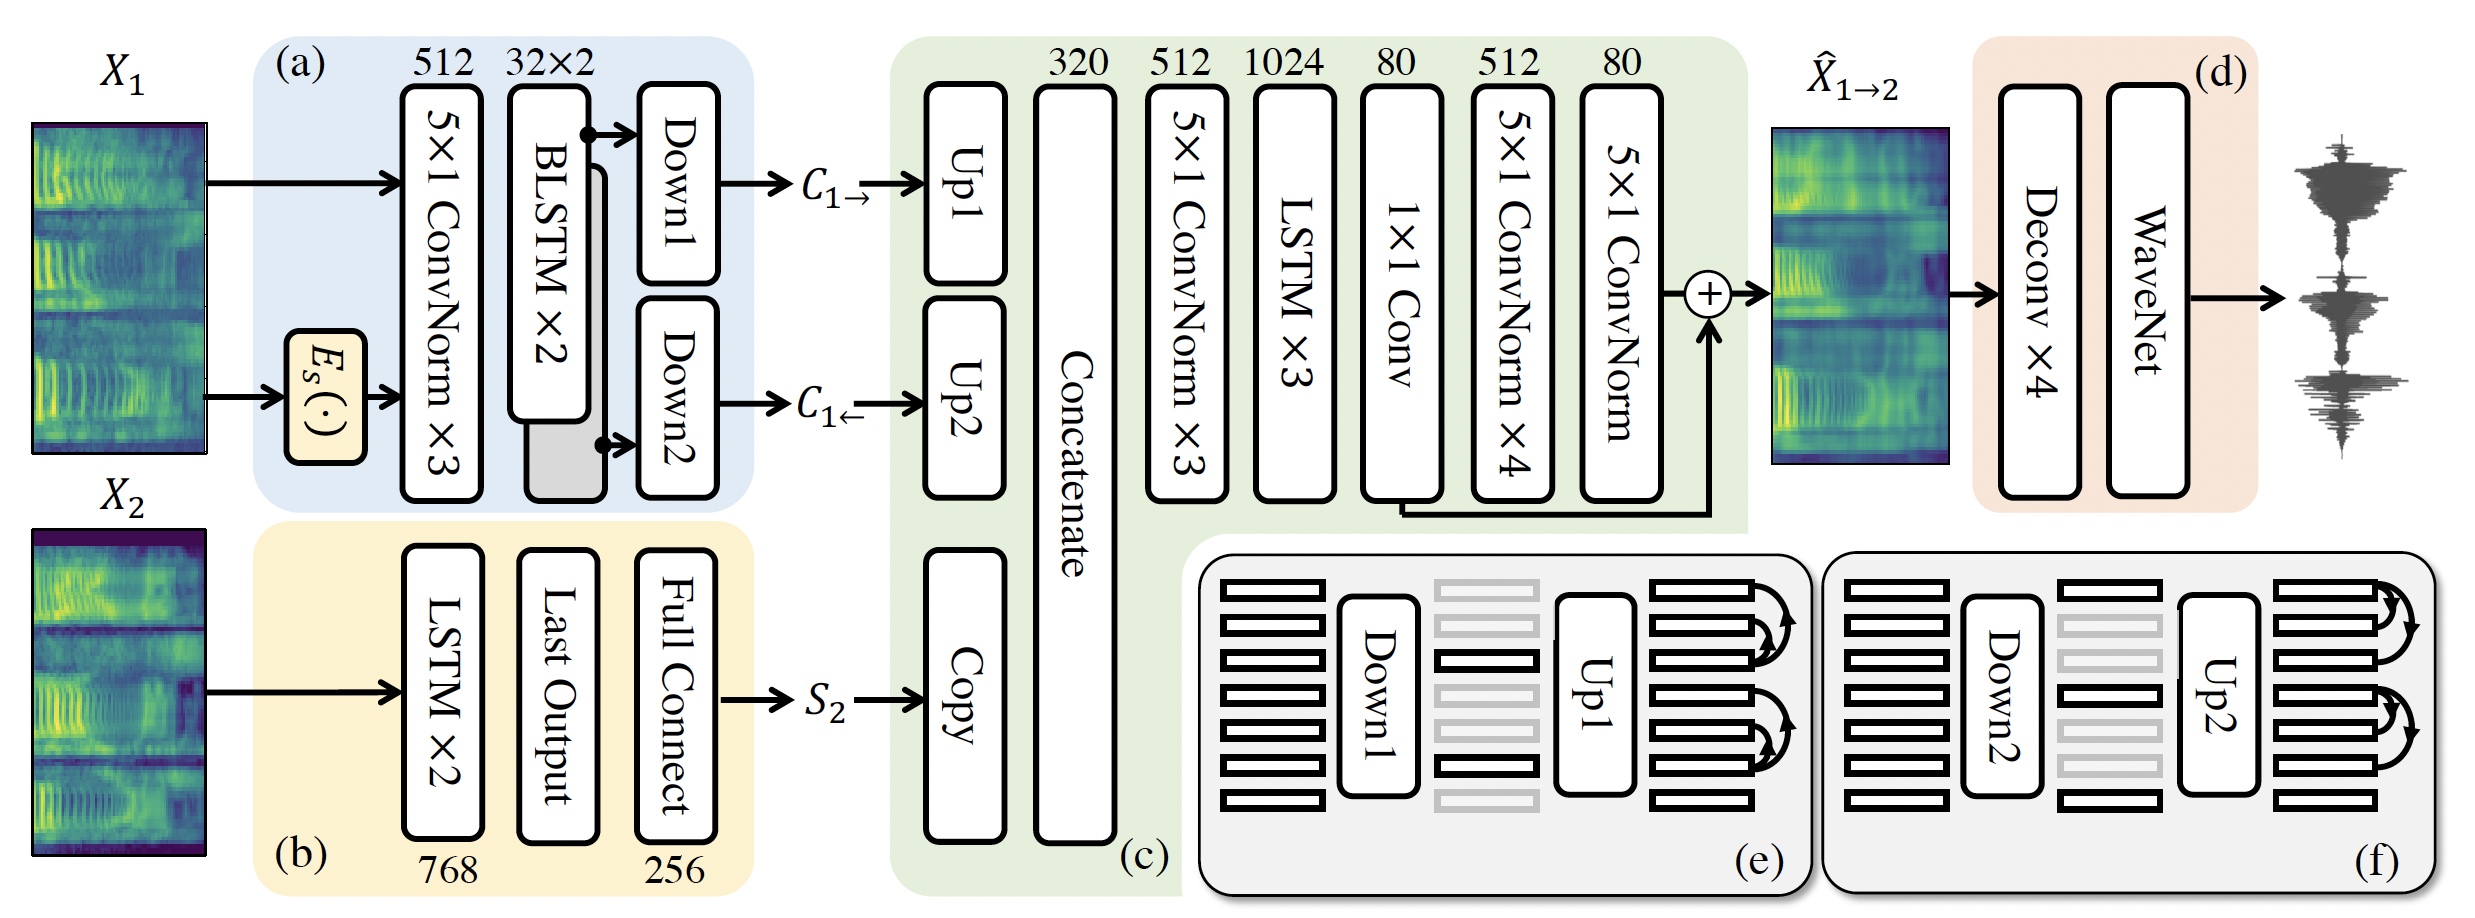
\includegraphics[width=\textwidth]{figs/qianfig3.png}}
\end{frame}

\begin{frame}
  \frametitle{Zero-Shot Voice Conversion}

  Since AutoVC represents the target speaker using a d-vector, it can
  be used to convert speech into the voice of somebody it never heard
  during training (``zero-shot voice conversion'').  Here are some
  examples:

  \centerline{\url{https://auspicious3000.github.io/autovc-demo/}}

\end{frame}

%%%%%%%%%%%%%%%%%%%%%%%%%%%%%%%%%%%%%%%%%%%%%%%%%%%%%%%%%
\section{Conclusions}
\setcounter{subsection}{1}

\begin{frame}
  \frametitle{Conclusions: Autoencoders}

  \begin{itemize}
  \item An autoencoder converts $\bm{x}$ into $\bm{h}$ such that
    $\text{len}(\bm{h})<\text{len}(\bm{x})$, but $\bm{h}$ contains
    most of the information in $\bm{x}$, in the sense that it
    minimizes $\Vert\bm{x'}-\bm{x}\Vert^2$.
  \item A linear autoencoder finds PCA.  The linear autoencoder is
    called ``smart PCA'' because, if
    $\text{len}(\bm{h})\ll\text{len}(\bm{x})$, training the neural net
    may be less computationally expensive than finding the
    eigenvectors of the covariance.
  \item A sparse autoencoder permits at most $K$ elements of $\bm{h}$
    to be nonzero, and therefore achieves zero error if $\bm{x}$ is
    drawn from a $K$-dimensional sparse manifold.
  \item A deep autoencoder finds $\bm{z}=f(\bm{x})$, a nonlinear
    transformation of $\bm{x}$, and is able to represent $\bm{x}$ with
    nonzero error if $\bm{x}$ is drawn from a
    $\text{len}(\bm{z})$-dimensional nonlinear manifold.
  \item An LSTM autoencoder can convert between sequences of different lengths.
  \end{itemize}
\end{frame}

\begin{frame}
  \frametitle{Conclusions: Voice Conversion}

  \begin{itemize}
  \item Supervised voice conversion assumes that you have paired
    utterances, in which source and target speaker say the same thing.
    \begin{itemize}
    \item One-to-one: one source speaker, one target speaker.
    \item Many-to-many: target speaker is specified by a speaker-ID
      vector, e.g., a d-vector.  System is trained to generate a voice
      given its d-vector.
    \end{itemize}
  \item Zero-shot voice conversion assumes that the target speaker was
    not part of the training dataset.
    \begin{itemize}
    \item AutoVC is trained using self-conversion, i.e.,
      $\bm{X}_{1\rightarrow{1}}=D(\bm{C}_1,\bm{S}_1)$.
    \item The speaker code is a speaker-ID system, e.g., d-vector.
    \item If speaker verification can tell who the source speaker was, then reduce the
      bottleneck dimension and try again.
    \item If reconstruction error rate is too high, then increase the
      bottleneck dimension and try again.
    \end{itemize}
  \end{itemize}
\end{frame}

\end{document}

